\documentclass[11 pt]{exam}

\usepackage{amsmath, amsfonts, color, tikz, bbm, txfonts, euscript}
\usepackage{amssymb}
\usepackage{enumerate}

\usepackage{pgfplots}
\usepackage{polynom}

\usetikzlibrary{calc}

\pagestyle{head}\headrule

\firstpageheader{Math 152}{\textbf{Challenge 1}}{}

\runningheader{Math 152}{\textbf{Challenge 1}}{}

\bracketedpoints

%\printanswers

\shadedsolutions\definecolor{SolutionColor}{rgb}{1,1,1}                                   

%The addpoints command makes the \numpoints command available.  Do not comment if you plan to keep this in the header.
%\addpoints
\begin{document}

\begin{center}
\fbox{\fbox{\parbox{5.5in}{\centering
\textbf{Read each question carefully and be sure to \textbf{SHOW ALL WORK}. Pa\c{c} fat! Good luck!} }}}    
\end{center} 

\vspace{0.15in}
\hbox to \textwidth{Name:\enspace\hrulefill}
\vspace{0.2in}

\vspace{0.15in}
\begin{questions}



\question[24] Use the sketch below of the graph of $y = f(x)$ on the interval $[-4,5]$ and answer the following questions using geometric arguments such as formulas of areas from geometry, properties of definite integrals, or the Fundamental Theorem  of Calculus.

\begin{center}

	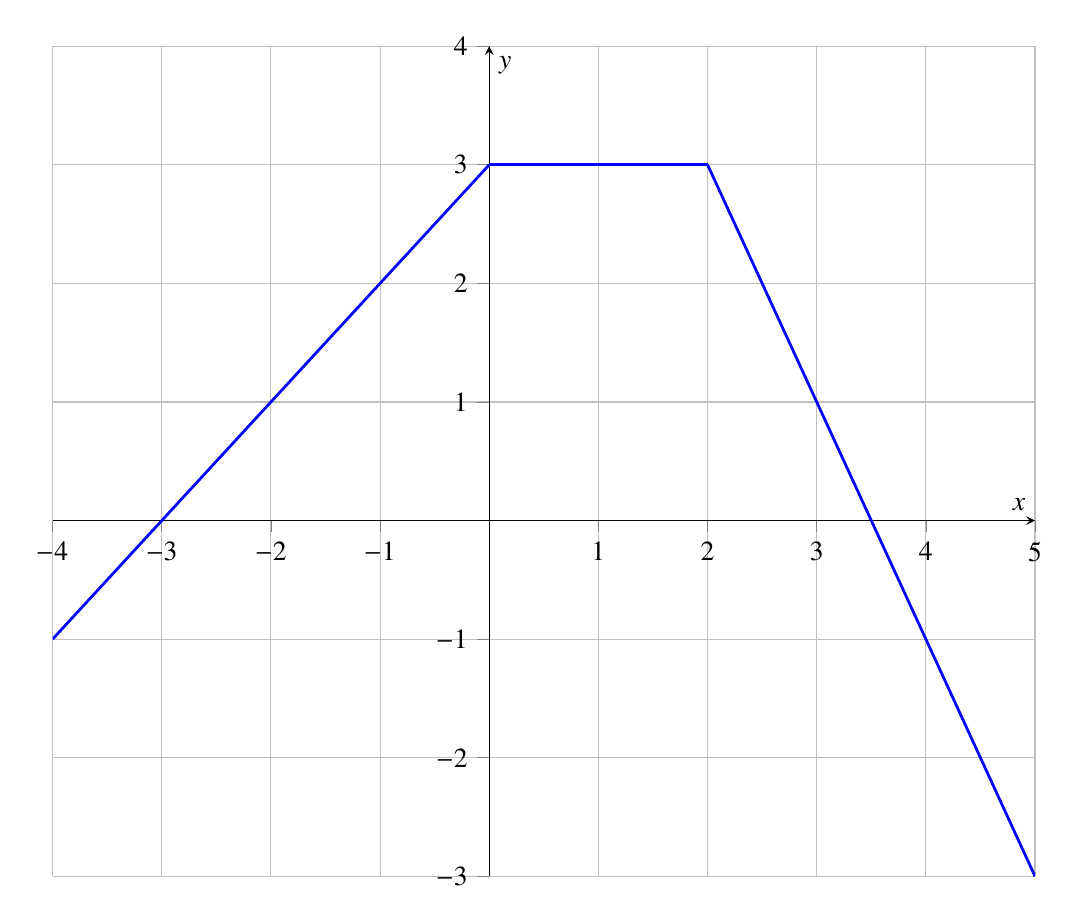
\begin{tikzpicture}

			\begin{axis}[xmin=-4,
						 xmax=5,
						 ymin=-3,
						 ymax=4,
						 width=400pt,
						 xlabel=$x$,
						 ylabel={$y$},
						 axis x line=middle,
						 axis y line=center,
						 tick align=outside,
						 grid=major]
						 				 
			\addplot[domain=-4:0,
						 line width=1pt,
						 no markers,
						 solid,
						 blue, samples=500] {3+x};	
			
			\addplot[domain=0:2,
			line width=1pt,
			no markers,
			solid,
			blue, samples=500] {3};
			
			\addplot[domain=2:5,
			line width=1pt,
			no markers,
			solid,
			blue, samples=500] {7-2*x};
			
			
			\end{axis}
	
	\end{tikzpicture}
	
\end{center}

\begin{enumerate}[(a)]


\item $\displaystyle \int_{-1}^{2} f(x) dx = $\\

\begin{solution}[0.3in]

\end{solution}

\item $\displaystyle \int_{5}^{-4} f(x) dx = $\\

\begin{solution}[0.3in] 
\end{solution}


\item $\displaystyle \int_{-4}^{5} 2f(x) dx = $\\

\begin{solution}[0.3in]

\end{solution}

\item $\displaystyle \int_{1}^{3} f(x)-2 dx = $\\

\begin{solution}[0.3in]
\end{solution}

\item If $A(x) = \displaystyle \int_{-2}^{x} f(t) dt,$ then $A(-2) = $.\\

\begin{solution}
\end{solution}

\item If $A(x) = \displaystyle \int_{-2}^{x} f(t) dt,$ then $A'(-2) = $.\\

\begin{solution}
\end{solution}

\end{enumerate}


 \question[20] Approximate $\displaystyle \int_{0}^2 x^{1/3} dx$ with 5 rectangles using any Riemann sum you wish. Then write this computation down using the sigma summation notation. Make sure to draw a sketch of the function and the rectangles. 
 
 \begin{solution}[3in]
 \end{solution}
 
 
 \question[20]  Let $\displaystyle F(x) = \int_{-5}^x 3t^2 dt$. Find the following.
 
 
 \begin{enumerate}[(a)]
 	
 	\item $F(-5) = $
 	
 	\hfill \break
 	
 	\item $F\rq{}(x) = $\\
 	
 	\item $F\rq{}(\pi) = $
 	
 	\hfill \break
 	
 	\item $\displaystyle \frac{d}{dx}\left(F(\cos(x))\right) = $
 	
 	\hfill \break
 	
 	
 	\item $F(1) = $
 	
\newpage
 	
 \end{enumerate}
 
 \question[12] Let $v(t)$ be the velocity of a particle moving in a straight path on $[0,6]$. Assume that the position $S(t)$ of the particle was 0 units at the start, i.e., $S(0) = 0$. 
 
 \begin{center}
 	
 	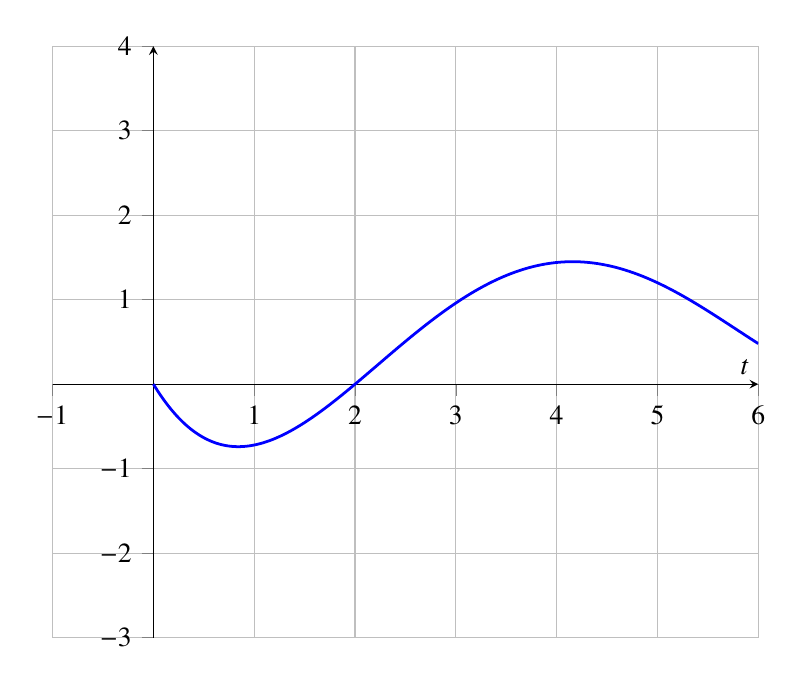
\begin{tikzpicture}
 	
 	\begin{axis}[xmin=-1,
 	xmax=6,
 	ymin=-3,
 	ymax=4,
 	width=300pt,
 	xlabel=$t$,
 	%ylabel={$f(t)$},
 	axis x line=middle,
 	axis y line=center,
 	tick align=outside,
 	grid=major]
 	
 	\addplot[domain=0:6,
 	line width=1pt,
 	no markers,
 	solid,
 	blue, samples=500] {x*(x-2)*(x-7)^2/50};	
 	
 	
 	
 	\end{axis}
 	
 	\end{tikzpicture}
 	
 \end{center}
 
 \begin{enumerate}[(a)]
 	
 	
 	\item At what time was the particle the furthest away from the starting point? How far is that approximately?
 	
 	\hfill \break
 	\hfill \break
 	\hfill \break
 	\hfill \break
\hfill \break
\hfill \break 	
 	
 	\item Describe when is $S(t)$ increasing, decreasing, concave up, or concave down on the interval $[0,6]$.
 	
 	\hfill \break
 	\hfill \break
 	\hfill \break
  	\hfill \break
 \hfill \break
 \hfill \break	
 	
 \end{enumerate}


\question[16] Evaluate the following definite integrals using geometry and the properties of definite integrals.

\begin{enumerate}[(a)]
	
	
	\item $\displaystyle \int_{0}^{3} |x-2| dx = $\\

	
	\hfill \break
	\hfill \break
	\hfill \break
	
	\newpage
	
		\item $\displaystyle \int_{-3}^{3}\sqrt{9-x^2} + 2x dx = $\\

	\hfill \break
\hfill \break
\hfill \break
	\hfill \break
\hfill \break
\hfill \break	
	\hfill \break
\hfill \break
\hfill \break	
\end{enumerate}

\question[4] You want to estimate the area underneath the graph of a positive function by using four rectangles of equal width. The rectangles that must give the best estimate of this area are those with height obtained from the:


\begin{enumerate}[(a)]
	
	\item Left endpoints of each interval
	
	\item Midpoints endpoints of each interval
	
	\item Right endpoints of each interval
	
	\item Not enough information
	
\end{enumerate}

\vfill

\question[4] A sprinter practices by running various distances back and forth in a straight line in a gym. Her velocity at $t$ seconds is given by the function $v(t)$. What does $\int_{0}^{60} |v(t)| dt$ represent?

\begin{enumerate}[(a)]
	
	\item The sprinter\rq{}s displacement from the starting point after one minute.
	\item The total distance the sprinter ran in one minute.
	\item The sprinter\rq{}s average velocity in one minute.
	\item None of the above.
	
\end{enumerate}

\vfill

\end{questions}

\end{document}
